%\begin{frame}{Discrimination of Photon Added States}{Noisy PACS discrimination: OOK}
%    \begin{center}
%        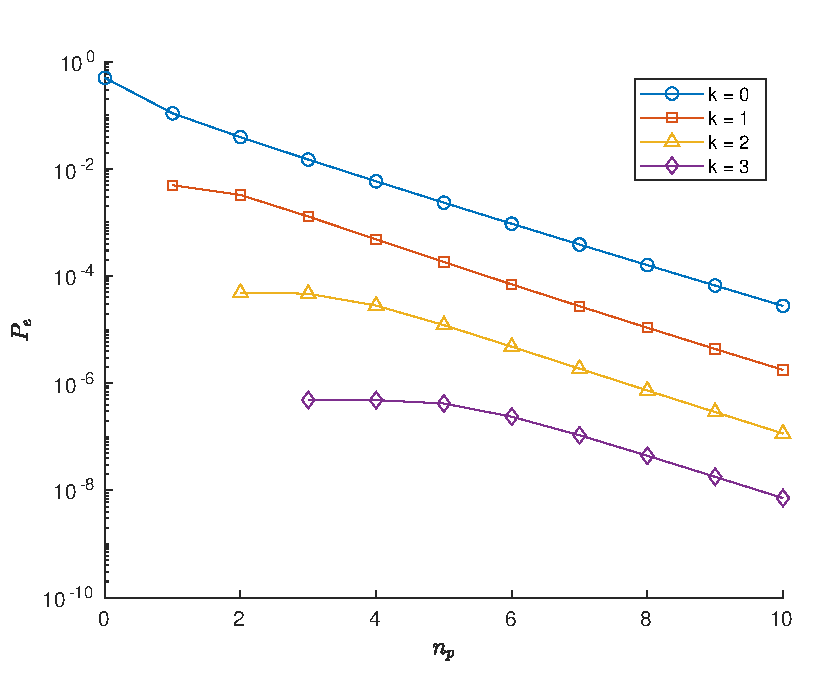
\includegraphics[width=0.65\textwidth]{Pictures/fig3.1.pdf}\\
%        \scriptsize{
%        MDEP of a QOOK system with PACS in terms of the mean photon number $n_p$.\\
%        $k=0,1,2,3$; $N=30$; $\bar{n}=10^{-2}$; $p_0=p_1=1/2$
%        }
%    \end{center}
%\end{frame}

\begin{frame}{Discrimination of Photon Added States}{Noisy PACS discrimination}
    \begin{center}
        %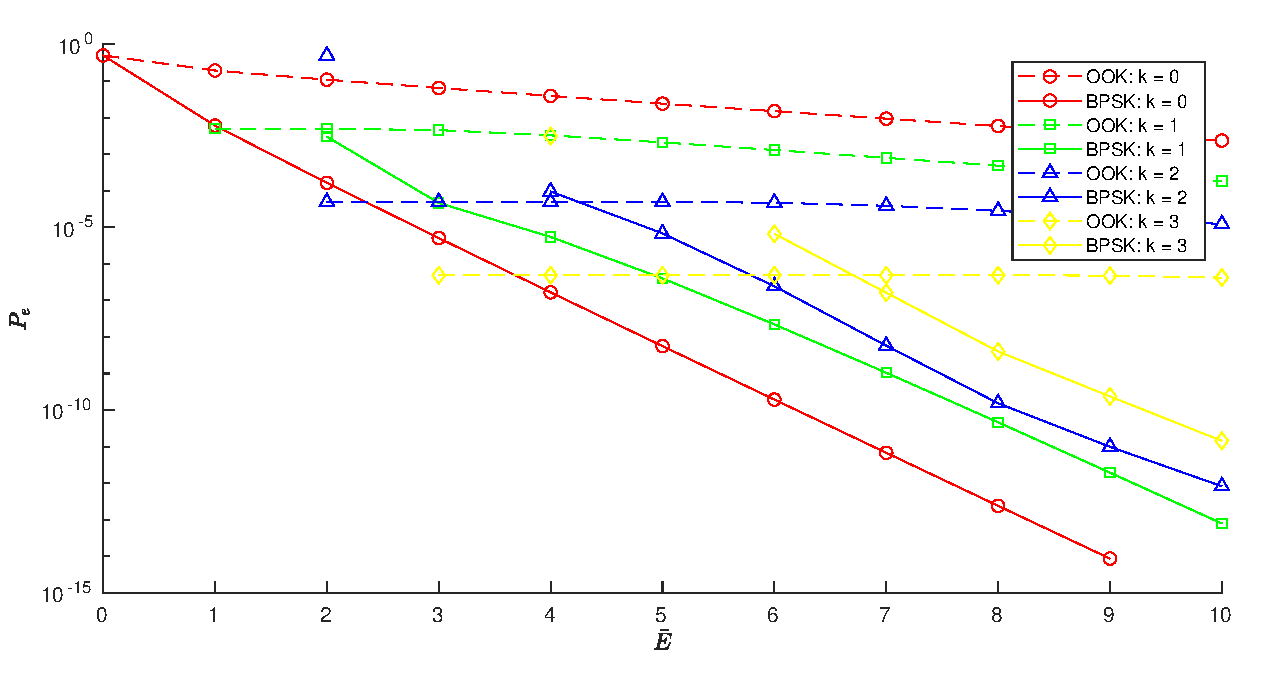
\includegraphics[width=0.9\textwidth]{Pictures/fig3.4.pdf}\\
        \resizebox{0.9\textwidth}{!}{
            % This file was created by matlab2tikz.
%
%The latest updates can be retrieved from
%  http://www.mathworks.com/matlabcentral/fileexchange/22022-matlab2tikz-matlab2tikz
%where you can also make suggestions and rate matlab2tikz.
%
\definecolor{mycolor1}{rgb}{0.00000,0.44706,0.74118}%
\definecolor{mycolor2}{rgb}{0.00000,0.45098,0.74118}%
\definecolor{mycolor3}{rgb}{0.85098,0.32549,0.09804}%
\definecolor{mycolor4}{rgb}{0.92941,0.69412,0.12549}%
\definecolor{mycolor5}{rgb}{0.49412,0.18431,0.55686}%
%
\begin{tikzpicture}

\begin{axis}[%
width=6.483in,
height=3.829in,
at={(1.087in,0.517in)},
scale only axis,
unbounded coords=jump,
xmin=0,
xmax=10,
xlabel style={font=\color{white!15!black}},
xlabel={$\bar{n}_p$},
ymode=log,
ymin=1e-15,
ymax=1,
yminorticks=true,
ylabel style={font=\color{white!15!black}},
ylabel={$P_e$},
axis background/.style={fill=white},
axis x line*=bottom,
axis y line*=left,
legend style={at={(0.137,0.117)}, anchor=south west, legend cell align=left, align=left, draw=white!15!black}
]
\addplot [color=mycolor1, dashed, line width=1.0pt, mark=o, mark options={solid, mycolor1}]
  table[row sep=crcr]{%
0	0.5\\
0.5	0.108700458264773\\
1	0.0390589952204486\\
1.5	0.0149211944183797\\
2	0.00585810811660947\\
2.5	0.00234016700918721\\
3	0.000947208632004815\\
3.5	0.000387493709571696\\
4	0.000159914025619767\\
4.5	6.64741197599072e-05\\
5	2.77990948747697e-05\\
5.5	1.1684045706617e-05\\
6	4.93169425797024e-06\\
6.5	2.08910579063692e-06\\
7	8.87685091988111e-07\\
7.5	3.78186394311975e-07\\
8	1.61491256200907e-07\\
8.5	6.90975989203757e-08\\
9	2.96172678604378e-08\\
9.5	1.27148974682356e-08\\
10	5.4664553994499e-09\\
};
\addlegendentry{OOK: k = 0}

\addplot [color=mycolor2, line width=1.0pt, mark=o, mark options={solid, mycolor2}]
  table[row sep=crcr]{%
0	0.5\\
0.5	0.04022904908515\\
1	0.00602305194817399\\
1.5	0.000973100923660764\\
2	0.00016419850351862\\
2.5	2.8533537561326e-05\\
3	5.0606940802389e-06\\
3.5	9.10735823422826e-07\\
4	1.65661779849557e-07\\
4.5	3.03786595323707e-08\\
5	5.60600271759526e-09\\
5.5	1.03974562293274e-09\\
6	1.93638272083518e-10\\
6.5	3.61866092646324e-11\\
7	6.78213041283016e-12\\
7.5	1.2740364319086e-12\\
8	2.40196751377653e-13\\
8.5	4.54081217071689e-14\\
9	8.65973959207622e-15\\
9.5	1.60982338570648e-15\\
10	0\\
};
\addlegendentry{BPSK: k = 0}

\addplot [color=mycolor3, dashed, line width=1.0pt, mark=square, mark options={solid, mycolor3}]
  table[row sep=crcr]{%
0	nan\\
0.5	0.0049504950495049\\
1	0.00326586474485618\\
1.5	0.00129261012790083\\
2	0.0004829624130685\\
2.5	0.0001823113671785\\
3	7.0042997465769e-05\\
3.5	2.73706278873798e-05\\
4	1.08587519096481e-05\\
4.5	4.36492203009786e-06\\
5	1.77428925313139e-06\\
5.5	7.28040018271869e-07\\
6	3.01099335797694e-07\\
6.5	1.25354203961425e-07\\
7	5.2479570245012e-08\\
7.5	2.20745764445418e-08\\
8	9.32266808195692e-09\\
8.5	3.95078869619425e-09\\
9	1.67926778038563e-09\\
9.5	7.15629389080874e-10\\
10	3.05683645063226e-10\\
};
\addlegendentry{OOK: k = 1}

\addplot [color=mycolor3, line width=1.0pt, mark=square, mark options={solid, mycolor3}]
  table[row sep=crcr]{%
0	nan\\
0.5	nan\\
1	0.499999999999999\\
1.5	0.0352896335380555\\
2	0.00299923864856155\\
2.5	0.000242653737939802\\
3	4.62511991632386e-05\\
3.5	1.64821131607429e-05\\
4	5.43086684001715e-06\\
4.5	1.55061238721332e-06\\
5	3.99663137751194e-07\\
5.5	9.60914410264024e-08\\
6	2.201131310553e-08\\
6.5	4.86964690793457e-09\\
7	1.04998582051152e-09\\
7.5	2.22034113317449e-10\\
8	4.6251891205884e-11\\
8.5	9.52177225954642e-12\\
9	1.94172455891817e-12\\
9.5	3.92685883809918e-13\\
10	7.91033905045424e-14\\
};
\addlegendentry{BPSK: k = 1}

\addplot [color=mycolor4, dashed, line width=1.0pt, mark=triangle, mark options={solid, mycolor4}]
  table[row sep=crcr]{%
0	nan\\
0.5	nan\\
1	4.90148024703263e-05\\
1.5	4.69619801760079e-05\\
2	2.81400977715229e-05\\
2.5	1.21516986146264e-05\\
3	4.80779255018771e-06\\
3.5	1.8744231199963e-06\\
4	7.33274078568158e-07\\
4.5	2.89379251172672e-07\\
5	1.15376949660906e-07\\
5.5	4.64708893033183e-08\\
6	1.88930928124442e-08\\
6.5	7.74504199663184e-09\\
7	3.19797588410609e-09\\
7.5	1.3287062561318e-09\\
8	5.55022250381398e-10\\
8.5	2.32915908782161e-10\\
9	9.81361103491452e-11\\
9.5	4.14942524784578e-11\\
10	1.76007541874412e-11\\
};
\addlegendentry{OOK: k = 2}

\addplot [color=mycolor4, line width=1.0pt, mark=triangle, mark options={solid, mycolor4}]
  table[row sep=crcr]{%
0	nan\\
0.5	nan\\
1	0.499999999999999\\
1.5	nan\\
2	0.499999999999999\\
2.5	0.0360954876474859\\
3	0.00276941242655876\\
3.5	0.000319766164387114\\
4	9.53611828535816e-05\\
4.5	2.83021512554327e-05\\
5	6.79567874584119e-06\\
5.5	1.37440529535127e-06\\
6	2.43371243435764e-07\\
6.5	3.88095893755214e-08\\
7	5.77702952142545e-09\\
7.5	8.68486338401198e-10\\
8	1.53136836544832e-10\\
8.5	3.53925222462692e-11\\
9	9.87959714038311e-12\\
9.5	2.88774559820126e-12\\
10	8.2261975009601e-13\\
};
\addlegendentry{BPSK: k = 2}

\addplot [color=mycolor5, dashed, line width=1.0pt, mark=diamond, mark options={solid, mycolor5}]
  table[row sep=crcr]{%
0	nan\\
0.5	nan\\
1	nan\\
1.5	4.85295073904268e-07\\
2	4.85188186849506e-07\\
2.5	4.18524906398154e-07\\
3	2.37374074729679e-07\\
3.5	1.07056314702092e-07\\
4	4.4415013722432e-08\\
4.5	1.79385606369209e-08\\
5	7.19588255648773e-09\\
5.5	2.89069451708812e-09\\
6	1.16715109799159e-09\\
6.5	4.74318695431464e-10\\
7	1.94059157632154e-10\\
7.5	7.99046939725656e-11\\
8	3.30934168957242e-11\\
8.5	1.37772571129346e-11\\
9	5.76222403125826e-12\\
9.5	2.41978659332176e-12\\
10	1.02018393732806e-12\\
};
\addlegendentry{OOK: k = 3}

\addplot [color=mycolor5, line width=1.0pt, mark=diamond, mark options={solid, mycolor5}]
  table[row sep=crcr]{%
0	nan\\
0.5	nan\\
1	nan\\
1.5	nan\\
2	0.499999999999999\\
2.5	nan\\
3	0.499999999999999\\
3.5	0.038524516196445\\
4	0.00310391579382863\\
4.5	0.000449655868986432\\
5	0.000129067667460958\\
5.5	3.28086831108965e-05\\
6	6.62678014318185e-06\\
6.5	1.10667807207143e-06\\
7	1.61993491565315e-07\\
7.5	2.33065918231468e-08\\
8	4.01583000186889e-09\\
8.5	9.11784814316974e-10\\
9	2.36422659227742e-10\\
9.5	6.03608274474254e-11\\
10	1.43704492749919e-11\\
};
\addlegendentry{BPSK: k = 3}

\end{axis}

\begin{axis}[%
width=8.365in,
height=4.698in,
at={(0in,0in)},
scale only axis,
xmin=0,
xmax=1,
ymin=0,
ymax=1,
axis line style={draw=none},
ticks=none,
axis x line*=bottom,
axis y line*=left
]
\end{axis}
\end{tikzpicture}%
        }\\
        \scriptsize{
            BPSK and OOK comparison in terms of MDEP as function of $\bar{n}_p$ 
            with $N=45$, $\bar{n}=10^{-2}$, $p_0=p_1=1/2$.
        }
    \end{center}
    \ \mbox{}\\ \ \mbox{}\\
\end{frame}